% -*- coding: utf-8 -*-

\documentclass[a4paper,dvipdfmx]{jsarticle}
\usepackage{ascmac,alltt,txfonts,url}

\usepackage[dvipdfmx]{graphicx}
\usepackage{here}

\renewcommand{\ttdefault}{cmtt}
\renewcommand{\figurename}{図} 
\renewcommand{\tablename}{表} 
\DeclareMathAlphabet{\mathtt}{OT1}{cmtt}{m}{n}
\SetMathAlphabet{\mathtt}{bold}{OT1}{cmtt}{m}{n}
\setlength{\oddsidemargin}{0cm}
\setlength{\evensidemargin}{0cm}

\makeatletter

\newdimen\@mojihaba
\settowidth{\@mojihaba}{あ}

\def\tokushu#1{%
\def\tokushutitle{#1}%
\gdef\articleHeader{\hbox to\textwidth{\rule{3\@mojihaba}{1mm}%
\hbox{\small\bf\hskip1mm \tokushutitle}\leaderfill}}
}

\newdimen \JQ	\JQ .259817mm	%%%	\JQ/\Q = 10pt/9.62216pt
\newdimen \Q	\Q  .25mm	%%%	Quarter of 1mm

\def\JarticleHeader{\rule{\textwidth}{1mm}}%
\def\JarticleTitle{{\huge\bf\@title}}
\def\JarticleAuthor{\large\begin{tabular}[t]{@{}l}\@author\end{tabular}}
\newbox\@temptitlebox

\def\verse{\let\\=\@centercr 
 \list{}{\itemsep\z@ \itemindent -1.5em\listparindent \itemindent 
 \rightmargin\leftmargin\advance\leftmargin 1.5em}\item[]}
\let\endverse\endlist
\def\quotation{\list{}{\listparindent 1.5em
 \itemindent\listparindent
 \rightmargin\leftmargin \parsep 0pt plus 1pt}\item[]}
\let\endquotation=\endlist
\def\quote{\list{}{\rightmargin\leftmargin}\item[]}
\let\endquote=\endlist
\def\abstquotation{\list{}{\listparindent 1.5em
 \itemindent\listparindent
 \leftmargin 5mm
 \rightmargin\leftmargin \parsep 0pt plus 1pt}\item[]}
\let\endabstquotation=\endlist
\def\quote{\list{}{\rightmargin\leftmargin}\item[]}
\let\endquote=\endlist

\global\def\@maketitle{\newpage \null
\hbox{\vbox to193.5\Q{\baselineskip=10mm % 193.5\Q = 9*\baselineskip
\begin{flushleft}
\JarticleHeader
% following extra vskip together with baselineskip(10mm) will produce
% appropriate 10mm/6mm gap between the rule and title
% This assumes that title is typeset with 28Q(7mm) font, and baseline
% is set 1mm above the bottom of the font.
\setbox\@temptitlebox\hbox{JarticleTitle}\ifdim\wd\@temptitlebox>\textwidth\vskip2mm\else\vskip6mm\fi
\leftskip=5mm
\JarticleTitle
\vskip6mm % to leave 10mm gap between title and author
\JarticleAuthor
\end{flushleft}\vfil}}
%\JEabstInsert
  \begin{small}
    \begin{abstquotation}
      \Jabstcontent
    \end{abstquotation}
  \end{small}
}

\long\def\Jabstract#1{\global\long\def\Jabstcontent{\noindent\ignorespaces #1}}
\def\Jabstcontent{\relax}

\makeatother

\usepackage{fancyhdr}
\pagestyle{fancy}
\lhead{イントロダクション}
\rhead{}
\rhead{\thepage{}}
\cfoot{}
\renewcommand{\headrulewidth}{0.5pt}
\pagestyle{fancy}

\Jabstract{%
\\
FPGAで何ができるか,どうすればFPGAを使うことができるのか,の概略を俯瞰しましょう.
}

\begin{document}

\title{イントロダクション}
\author{}
\date{2019年 1月14日~~第3.0版}
\maketitle

\section{もし○○を制御したいけどソフトウェアじゃ難しい}
実験などのために,何かの入力を観測しながら,それに応じて何かの処理をする,という機会がありませんか?そのような場合,パソコンやマイコンで実装してみようとしても
\begin{itemize}
 \item モータやセンサをたくさんつなぎたいから100個くらい自由に使える入出力があればいいのに
 \item システムを乾電池1本で動作しないかなあ
 \item 決められた時間内できちんと処理を終わらせたい/繰り返したい
 \item 処理専用の特別な命令を実行できたら高速化できるのにな
 \item いくつもの処理を並行して実行できたらいいのにな
 \item 361ビットの値の演算が一発でできたらすっきり書けるのに
\end{itemize}
など,ソフトウェアではあと一息痒いところに手が届かず,歯痒い思いをしたことはないでしょうか.

\subsection{プロセッサがプログラムを実行する}
パソコンはもちろんのこと,今やテレビや携帯電話,自動車などのあらゆる製品の中でソフトウェアが動作しています.それらのソフトウェアは,実現したいアプリケーションや動作させる環境に応じて,さまざまなプログラミング言語で記述されています.たとえば,JavaScriptはWebアプリケーションを便利に華やかにしてくれますし,Cで記述されたプログラムはシステムを細やかに制御し,高速に動作させることができます.

近年のソフトウェアが動作する環境は,プログラミング言語やオペレーティング・システム,ライブラリなどにより上手に隠蔽されていますので,抽象化された世界の上でプログラムを書けるソフトウェア・エンジニアは,ハードウェアを意識することが少ないかもしれませんが,どのような言語を使ったプログラムでも,ハードウェアであるプロセッサで処理が実行されます.

たとえば,パソコン上で動作するソフトウェアはIntelのCore i7などのプロセッサの上で動作し,スマートフォンの上のソフトはARMプロセッサの上で動作しています.また,組み込み機器でも各種マイコンの上で処理が実行されています.一般に,マイコンは,演算装置に加え様々なデバイスを制御するためのI/Oコントローラを備えているためセンサの入力を読み取ったり,モーターを回したりといった処理をソフトウェアで操作できます.
「プロセッサ」や「マイコン」はデバイスそのものがアプリケーションに応じて変化するわけではなく,図\ref{fig:software_on_processor})のように,ソフトウェアによって処理させる内容をその時々で決めることができるため,幅広い用途に活用されています.

 \begin{figure}[H]
  \begin{center}
   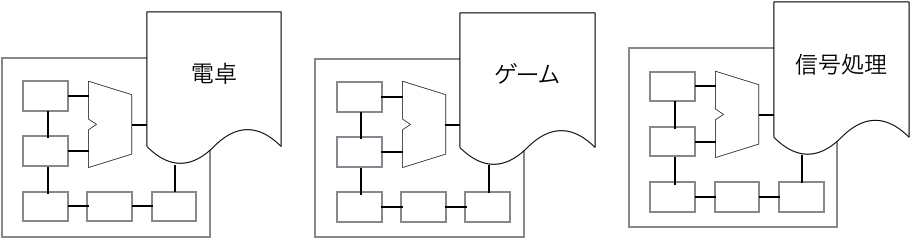
\includegraphics[width=.95\textwidth]{chapter01_figures/software_on_processor.png}
  \end{center}
  \caption{ソフトウェアプログラムはプロセッサの上で処理される.どんなプログラムを実行する場合でもプロセッサの構造は変わらない \label{fig:software_on_processor}}
 \end{figure}

一方で,自由に設計できるようにみえるソフトウェアも,実際に動作するときには,常にプロセッサの制約を受けます.たとえば,プロセッサの処理能力の限界を越えるような速さでの計算や,プロセッサがもっていないI/Oを操作するといったことはできません.
しかし,デバイスそのものをアプリケーションに応じて変化させて,冒頭に挙げたような「もし○○なプログラムが書けたなら」の希望を現実にできる手段があれば,今まで手を出しにくかったアプリケーションが実現できるのではないでしょうか.

\subsection{ハードウェア・デバイスを作るための便利な仕組み}
そんなときには,オリジナルのハードウェアを作るという解決策があります.ハードウェアを作るといっても,げじげじの足が付いたデバイスを一つずつはんだ付けしたり,半導体工場に製作を依頼する必要はありません.ハードウェア記述言語(HDL;Hardware Description Language)を用いて作成したハードウェア・イメージを専用のデバイス(FPGA)に書き込むだけでオリジナルのハードウェア・デバイスを作る便利な仕組みがあります.
FPGAは,図\ref{fig:fpga_simple_image}のように,論理回路になる素や,論理回路同士を接続する素がパッケージされたLSIです.

 \begin{figure}[H]
  \begin{center}
   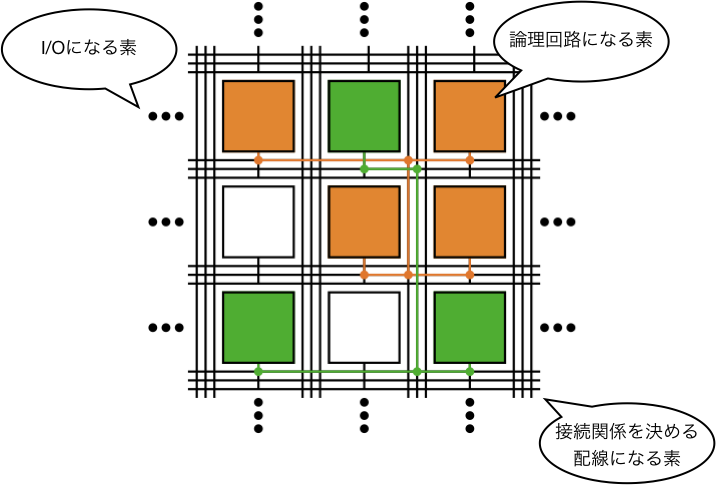
\includegraphics[width=.8\textwidth]{chapter01_figures/fpga_simple_image.png}
  \end{center}
  \caption{FPGAは,論理回路の素や配線回路の素がパッケージされたLSI \label{fig:fpga_simple_image}}
 \end{figure}

用途によって,とにかく短い時間で処理をしたい,低消費電力で処理をさせたい,同時にたくさんのI/Oにアクセスしたいといったことが求められることもあるでしょう.FPGAは,そんな要求に応えることができる,やりたい処理をさせるための専用ハードウェアを自在に作れる柔らかいプログラム可能なハードウェア・デバイスです(図\ref{fig:fpga_processing_image}).

 \begin{figure}[H]
  \begin{center}
   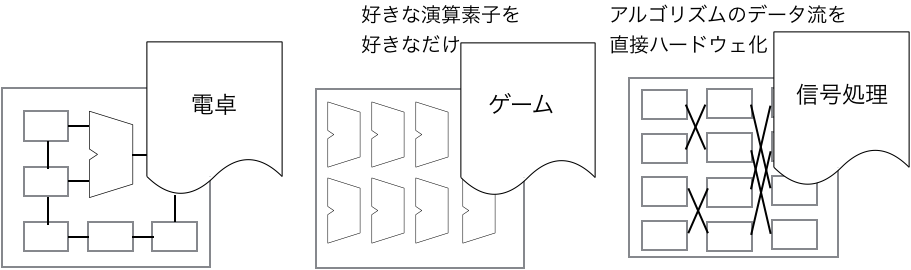
\includegraphics[width=.95\textwidth]{chapter01_figures/fpga_processing_image.png}
  \end{center}
  \caption{FPGAは,実現したい処理向けの専用ロジックを自分で作ることができる \label{fig:fpga_processing_image}}
 \end{figure}

\subsection{FPGAには小さなメモリ(LUT)がたくさん入っている}
FPGAの中身はどのようになっているのか,もう少し詳しくのぞいてみましょう.図\ref{fig:inside_fpga_example}は,代表的なFPGAメーカーであるXilinxとIntelのFPGAの内部構造です.多少違いはありますが,基本的な構成要素は,LUT(Look-up Table)と記憶素子(D-FF)で構成されるロジック・セルです.

 \begin{figure}[H]
  \begin{center}
   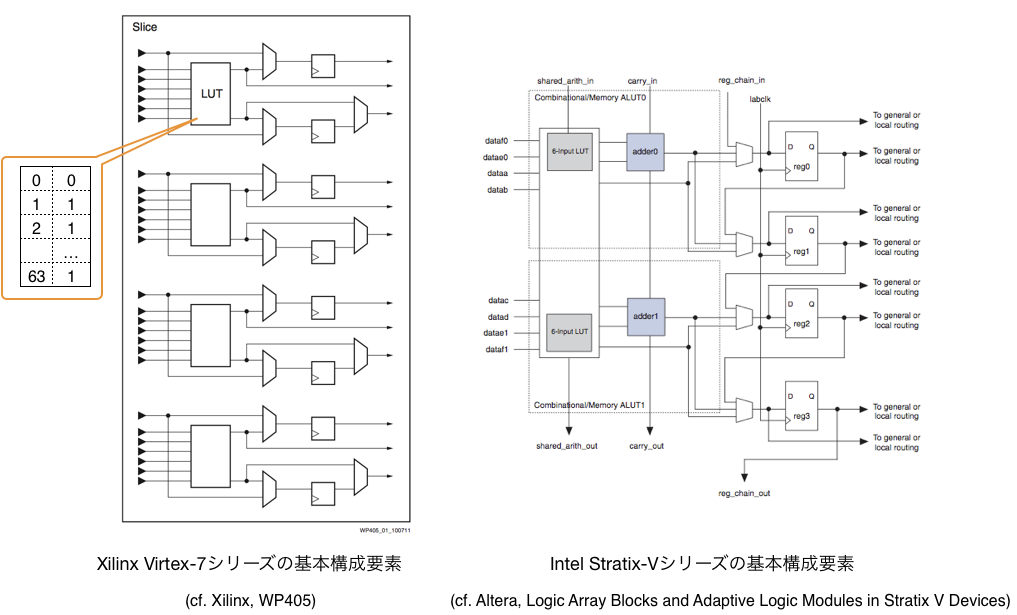
\includegraphics[width=.95\textwidth]{chapter01_figures/inside_fpga_example.png}
  \end{center}
  \caption{FPGAの内部構造 \label{fig:inside_fpga_example}}
 \end{figure}

好きな論理演算を実現する鍵はLUTで,これは小規模なメモリのようなものです.入力されたデータに対して出力する信号を決定するためのテーブルの役割を持ちます.

たとえば,図\ref{fig:inside_fpga_example}のように,アドレス0に0,それ以外のアドレス1〜63には,1と書いてあるLUTの場合には,6入力1出力のOR回路に相当します.同様に,アドレス0〜62に0をアドレス63に1と書いておけば,6入力1出力のAND回路を作ることができます.また,1が奇数個のアドレス,たとえば,アドレス1,2,4,7など,のみに1と書いておけば,6入力1出力のXOR回路になります.

入力ビット幅の範囲で好きな論理演算を決められるLUTと,複数のLUTを好きに接続できる接続テーブルによって,大規模な論理演算を好きに構成することができますね.

\subsection{ハードウェアと記述言語}

LUTと接続テーブルを設定して,ハードウェアを自由に設計できるといっても,ソフトウェアでは簡単に書ける足し算や引き算といった基本的な演算を,一つ一つ論理回路で構成するのは骨が折れる作業です.そこで利用するのがハードウェア記述言語(HDL; Hardware Description Language)です.

HDLは,Cプログラミングなどと同じように変数への加減算や条件分岐などを用いてハードウェアを設計できるプログラミング言語です.ユーザは,まるでプログラムをロードするように,ハードウェア・データをFPGAに書き込むことで所望のデバイスを作ることができます.

\section{ハードウェア・プログラミングを理解する三つのポイント}

オリジナルのハードウェアを作成するための手段が,ハードウェア・プログラミングです.ソフトウェア・プログラミングでは,プロセッサ(というハードウェア)を動作させるための命令列を設計するのに対し,ハードウェア・プログラミングは,ハードウェアそのものを設計します.ハードウェア・プログラミングにチャレンジするにあたり,ハードウェアの基本概念となる「演算の決め方」と「データの単位」,「処理の動作方式」についてソフトウェア・プログラミングと比較しながら説明します.

\subsection{演算の決め方}
ソフトウェア・プログラミングでは,演算はプロセッサのもつ命令として決められています.一方でハードウェア・プログラミングでは,論理演算を組み合わせて自分で演算を決めることができます.

\paragraph{ソフトウェア・プログラミング}
ソフトウェア・プログラミングは,プロセッサの演算ユニットが持つ機能をどのように利用するかを指示します.プロセッサの演算ユニットでは,足し算や掛け算などの算術演算や,比較演算,分岐などの処理を制御する命令を実行できます.また,信号処理を高速に処理できるように「掛け算して足し算」するといった命令を備えているプロセッサもありあます.実際にプロセッサの演算ユニットをどのように使うか,を決定するのはコンパイラの仕事で,プログラマは,普段ほとんど意識する必要はありません.

\paragraph{ハードウェア・プログラミング}
ハードウェア・プログラミングは,ハードウェアそのものを作成するので,ベースとなる演算ユニットというものは存在しません.演算処理は,基本的には,NOT,AND,ORの論理演算とそれらの組み合わせで実現します.

\subsection{データの単位}
ソフトウェア・プログラミングとハードウェア・プログラミングで取り扱い可能なデータの単位について比べてみます.

\paragraph{ソフトウェア・プログラミング}
一般に,プロセッサの作業領域であるレジスタの幅は固定されていて,ソフトウェア・プログラミングではそのサイズでしかデータを取り扱えません.たとえば,レジスタ幅が32ビットのプロセッサでは,1という値も4294967295という大きな値も32ビット幅のデータとして処理されます.また,512ビットという大きな値を取り扱うためには,512÷32の16回分のデータ処理を必要とします.

\paragraph{ハードウェア・プログラミング}
ハードウェア・プログラミングでは,‘0’または‘1’の値である1ビット単位のデータを自由に組み合わせて利用できます.処理内容によって,好きなビット数のデータを定義できるので,大きいデータも小さいデータも自由に定義して処理できます.512ビットのデータも,ハードウェア・プログラミングなら1回のデータ処理で取り扱えます.

\subsection{処理の動作方式}
ソフトウェア・プログラムは,プロセッサが記述した処理を順序よく実行してくれます.しかし,ハードウェア・プログラムは,生成されたハードウェア回路そのものがデータを処理します.そのため,処理の順序を守るための仕組みが必要な場合には自分でそのしくみを作る必要があります(図 \ref{fig:software_vs_hardware}).

 \begin{figure}[H]
  \begin{center}
   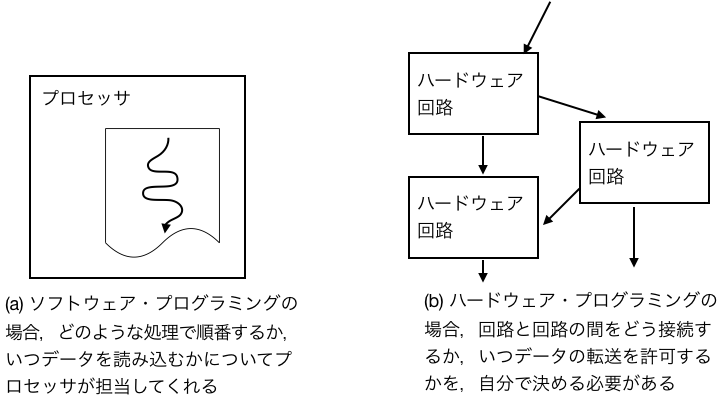
\includegraphics[width=.8\textwidth]{chapter01_figures/software_vs_hardware.png}
  \end{center}
  \caption{ソフトウェア・プログラミングではプロセッサが処理順序を決めてくれる.ハードウェア・プログラミングでは,ハードウェアを構成する回路同士の接続関係や,いつデータを転送するかを全部自分で決める必要がある.\label{fig:software_vs_hardware}}
 \end{figure}

\paragraph{ソフトウェア・プログラミング}

今日のプロセッサの基本的な構成方式は,図\ref{fig:processor_model_image}に示すノイマン型アーキテクチャと呼ばれる方式です.ノイマン型アーキテクチャがプログラムを実行する手順はおよそ次の通りです.
\begin{enumerate}
 \item 命令を読み込む
 \item 読み込んだプログラムの命令を理解する
 \item 演算ユニット上で命令を実行する
 \item 必要に応じてメモリを読み書きする
 \item 1.に戻る
\end{enumerate}
パソコンのプロセッサに見られる「クロック3GHz」といったスペックのプロセッサでは,プロセッサ内のユニットが3GHzのクロックに同期して,すなわち0.33n秒程度の時間で動作することで,このサイクルが繰り返されます.

 \begin{figure}[H]
  \begin{center}
   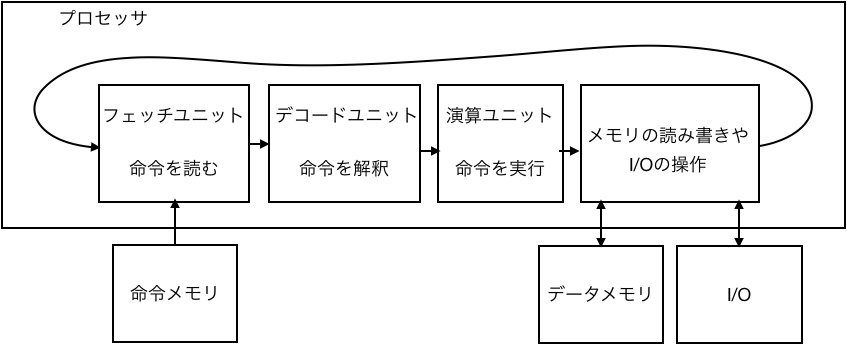
\includegraphics[width=.8\textwidth]{chapter01_figures/processor_model_image.png}
  \end{center}
  \caption{今日のプロセッサの典型的な構成方式.処理性能向上のために,各ユニットは可能な限り並行に動作するように工夫されることが多い.\label{fig:processor_model_image}}
 \end{figure}

命令を実行する,演算ユニットでは,決められたビット幅の作業領域の値に足し算や掛け算などの演算を適用できます.高い処理性能を達成するために,複数の演算ユニットを持つプロセッサもあり,それらのプロセッサでは,演算ユニットの個数分だけ同時に命令を処理することができます.勿論,「演算Aの後に演算Bを計算しないと演算Aの結果が保存されない,とか,演算Bの入力が揃う前に計算をはじめてしまう」ということは普通はなく,プロセッサが演算の順番を守ってくれます.

\paragraph{ハードウェア・プログラミング}

ハードウェアの基本となる論理演算回路において,入力信号を与えてから出力信号が得られるまでの時間は,トランジスタの特性や論理演算の段数で決定されます.そのため,複雑にゲートが関係し合うような回路で,データが正しく到達することを考慮するのは大変困難です(図\ref{fig:async_logic_timing}).

 \begin{figure}[H]
  \begin{center}
   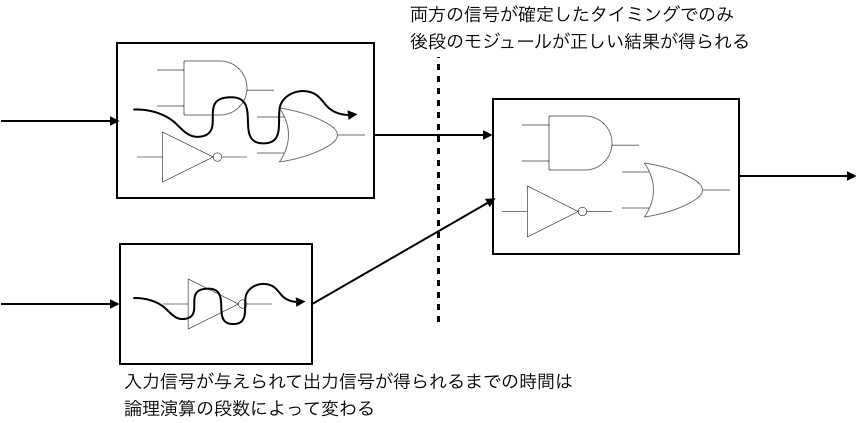
\includegraphics[width=.8\textwidth]{chapter01_figures/async_logic_timing.png}
  \end{center}
  \caption{入力された信号に対して出力が確定するまでの時間は,論理演算回路を構成する論理演算の段数で決まる.\label{fig:async_logic_timing}}
 \end{figure}

ハードウェア・プログラミングでは,これを解決するために大抵の場合,「同期順序回路」という構成方法を利用します.同期順序回路では,独立に動作するハードウェア中のモジュールのデータの入力のタイミングを,共通の信号「クロック」に合わせて制御します.ある単位処理を受けもつハードウェア・モジュールは,クロックが立ち上がりや立ち下がりから一定期間の間で必ず信号を読み取ることにします(図\ref{fig:sync_logic_timing}).全てのモジュールが,(1)クロックに間にあうように信号を決定し,(2)一定の期間値を変更しない,というルールさえ守れば,全体の演算が正しく動作します.

 \begin{figure}[H]
  \begin{center}
   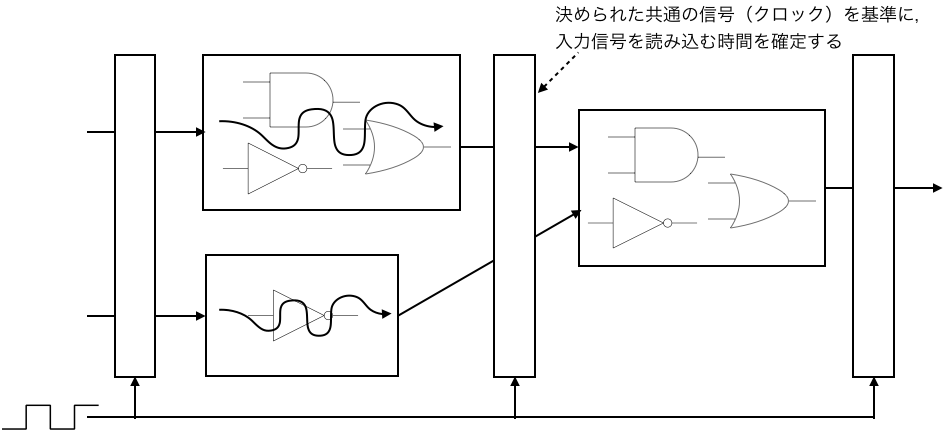
\includegraphics[width=.8\textwidth]{chapter01_figures/sync_logic_timing.png}
  \end{center}
  \caption{入力された信号に対して出力が確定するまでの時間は,論理演算回路を構成する論理演算の段数で決まる.\label{fig:sync_logic_timing}}
 \end{figure}


回路全体がクロックに合わせて動作するため,クロックの周期が短いほど全体が高速に動作します.しかし,やみくもにクロックを短くできるというわけではありません.

\section{ハードウェア・プログラミングの流れ - 使用する言語と必要なツールは?}
ハードウェア・プログラングの詳細は,以降の章で実例と共に紹介しますが,まずは全体の流れのイメージをつかんでみましょう.

FPGAを使ったハードウェア・プログラミングは,図\ref{fig:fpga_development_flow}のような流れで行ないます.流れ自体はソフトウェア・プログラミングとあまり変わりません.

 \begin{figure}[H]
  \begin{center}
   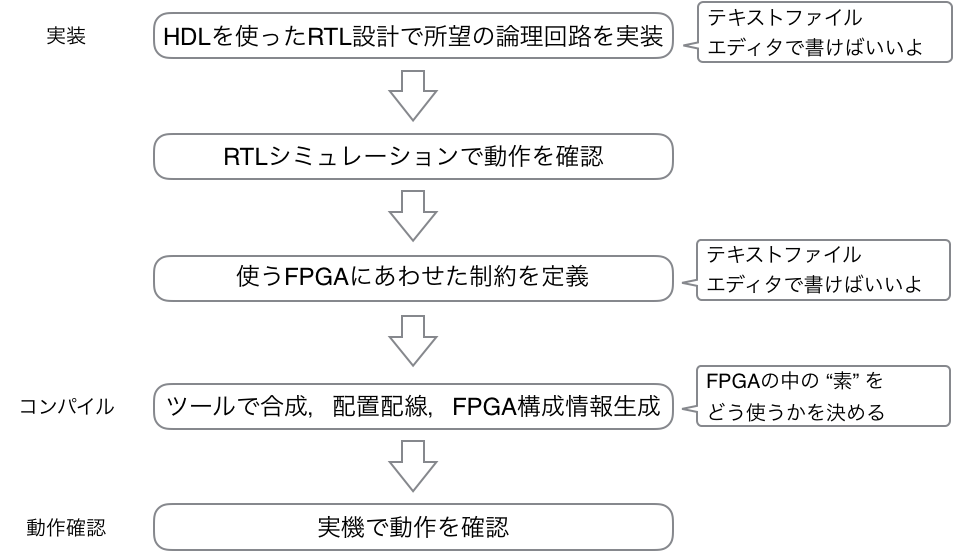
\includegraphics[width=.8\textwidth]{chapter01_figures/fpga_development_flow.png}
  \end{center}
  \caption{FPGAを使ったハードウェア・プログラミングの流れ.\label{fig:fpga_development_flow}}
 \end{figure}

ハードウェア・プログラミングには,ハードウェア記述言語(HDL; Hardware Description Language)を使用します.一般的に使用されているのは,VHDLとVerilog HDLの2種類です.記述自体は好きなテキストエディタで行なって構いません.図\ref{fig:writing_vhdl_example}は,emacsを使ってVHDLを記述している例です.

 \begin{figure}[H]
  \begin{center}
   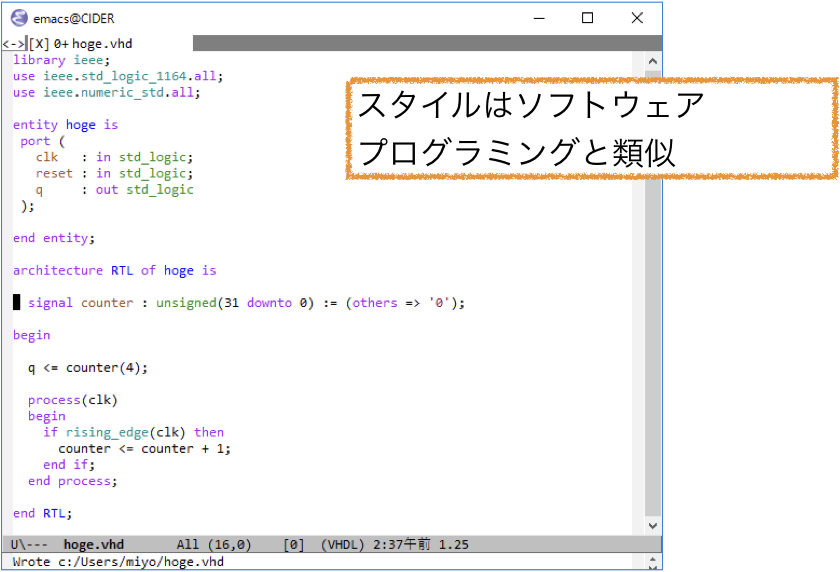
\includegraphics[width=.8\textwidth]{chapter01_figures/writing_vhdl_example.png}
  \end{center}
  \caption{emacsを使ってVHDLを記述している例.\label{fig:writing_vhdl_example}}
 \end{figure}

HDLでハードウェアを設計したら,正しく動作を記述できているかRTLシミュレーションというフローで確認します.コマンドラインベースで使える簡単なシミュレーションツールや,回路の動作の流れを信号の変化をグラフィカルに表示するツールなどがあります.図\ref{fig:simulation_image}は,図\ref{fig:writing_vhdl_example}で記述したハードウェアをシミュレーションし信号の変化を描画した様子です.

 \begin{figure}[H]
  \begin{center}
   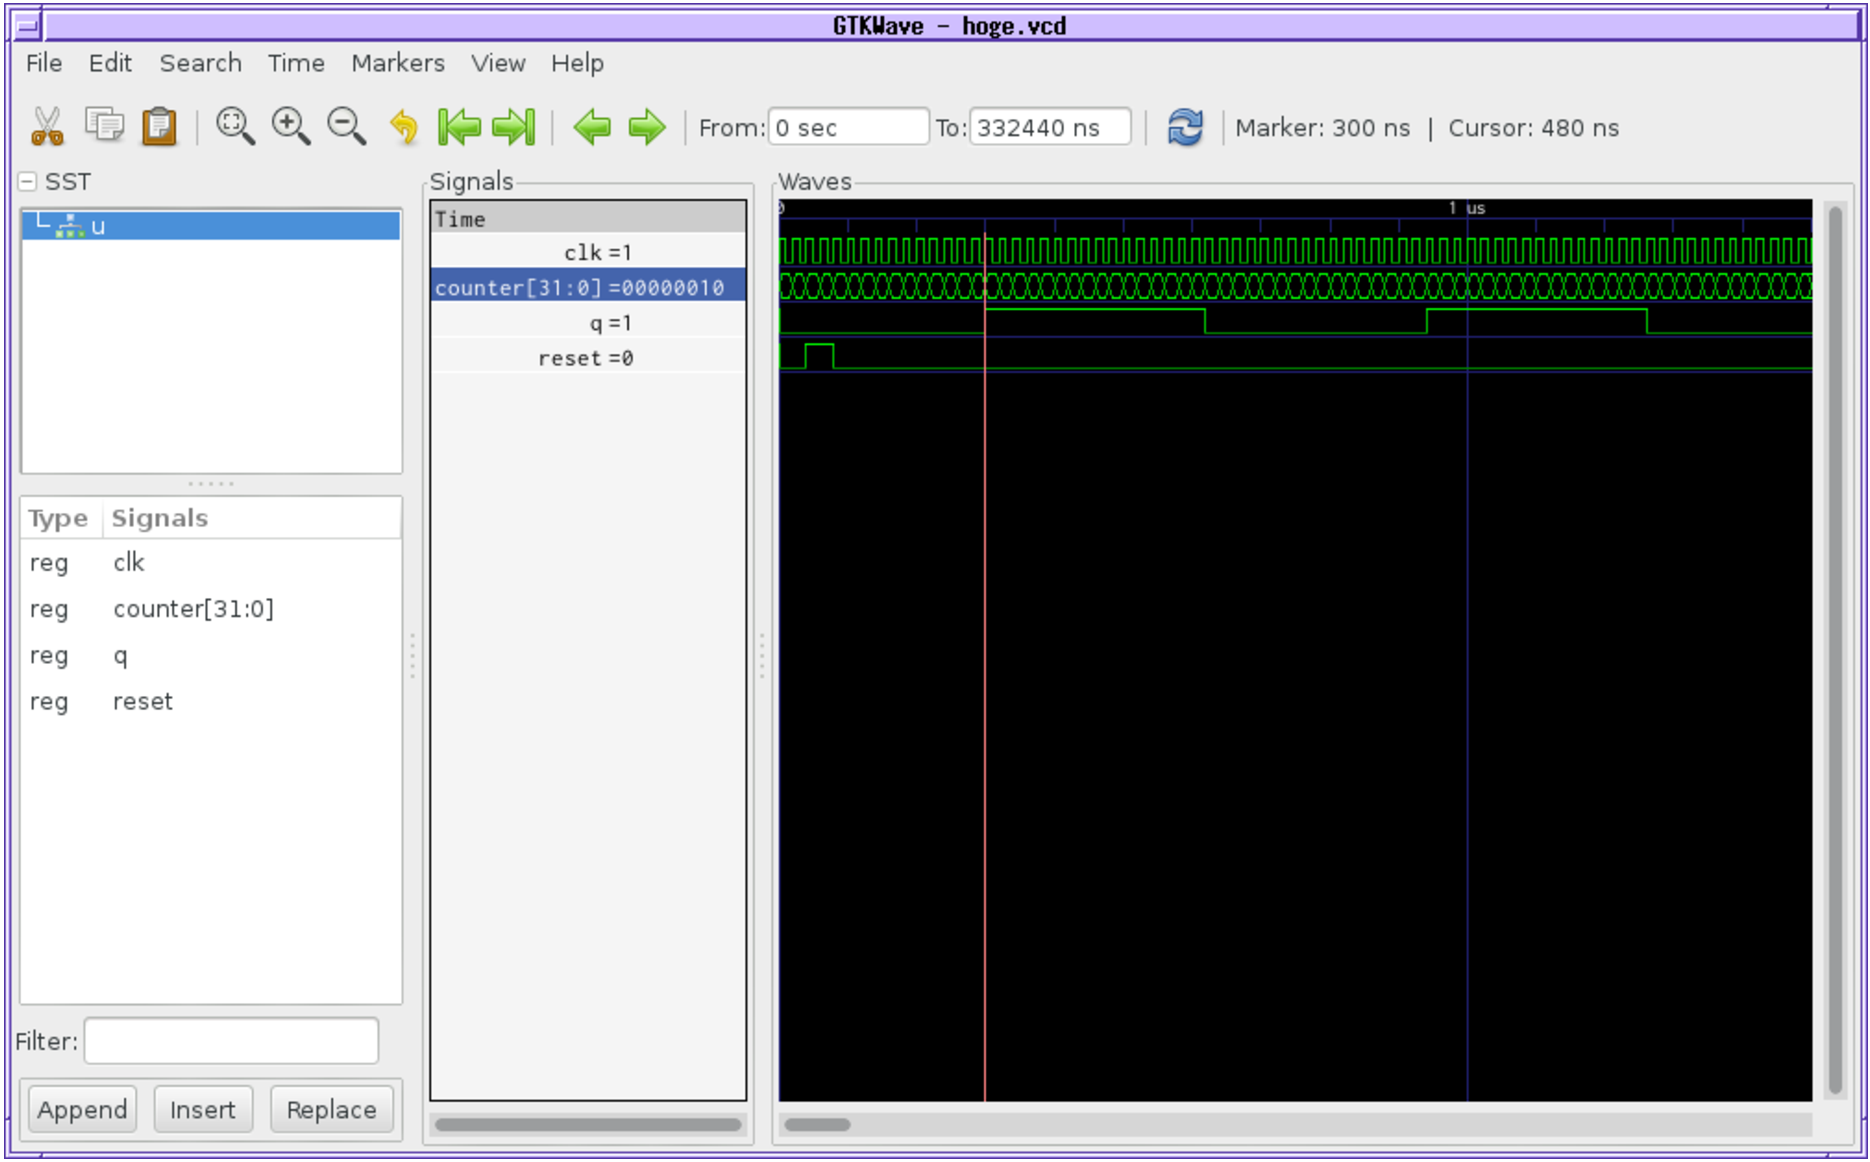
\includegraphics[width=.8\textwidth]{chapter01_figures/simulation_example.pdf}
  \end{center}
  \caption{シミュレーション結果を確認している様子.\label{fig:simulation_image}}
 \end{figure}


動作の確認ができたら,開発ツールの助けを借りてハードウェアに書き込む構成情報を生成します.開発ツールで行う作業は,合成と配置配線,構成情報生成の3段階です.必要なツールは,FPGAベンダである米国のIntel社とXilinx社の両方から,それぞれ専用のものが提供されています.また,最適化処理などに特色を持つサード・パーティ製の開発ツールもあり,必要に応じて使い分けるとよいでしょう.図\ref{fig:fpga_devtool_image}は,開発ツールの例です.

 \begin{figure}[H]
  \begin{center}
   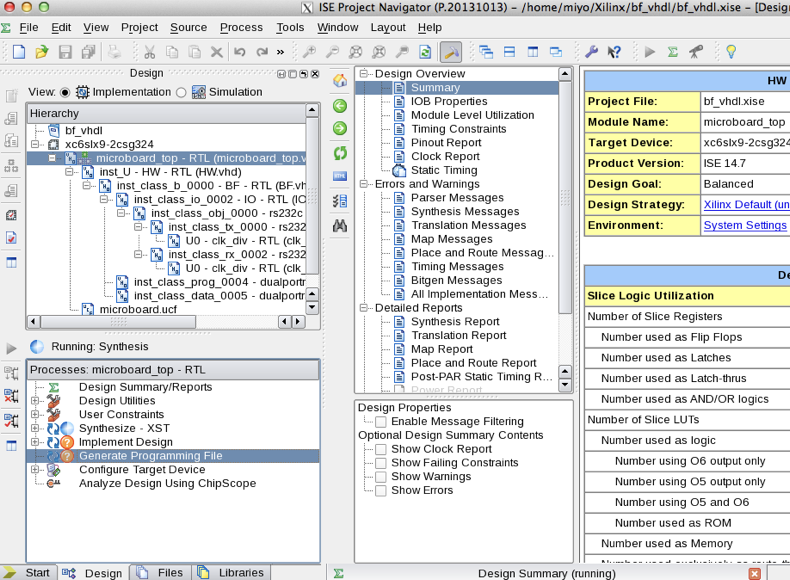
\includegraphics[width=.8\textwidth]{chapter01_figures/fpga_devtool_image.png}
  \end{center}
  \caption{開発ツールを使って,合成・配置配線・構成情報の生成を行なう.\label{fig:fpga_devtool_image}}
 \end{figure}

開発ツールの行う,ハードウェア・プログラミング特有の作業内容は次の通りです.
\begin{description}
 \item[合成 - 論理回路に置き換える処理] 記述されたHDLを解釈し,論理回路に置き換えます.また,さまざまな最適化を適用し,小さく高速な回路を自動で生成します.
 \item[配置配線 - ロジック・セルの割り当てと接続を決定] 合成して生成した論理回路をFPGA内にあるロジック・セルを組み合わせて実現するための割り当てと接続関係を決定します.ここで,ユーザが「特定の回路同士を近付ける」や,「特定の出力を好きなピンにアサインする」などの設定を与えられます.
 \item[構成情報生成- 書き込み用ファイルを作る] 最後にFPGAに書き込み可能な構成情報を生成します.
\end{description}
ソフトウェア・プログラミングであれば,コンパイル,リンク,バイナル生成に相当するステップだと思えばよいでしょう.

構成情報の生成が完了したら,そのデータを書き込みソフトウェアを使用してFPGAに書き込むことで設計したハードウェアを動かすことができます.

\section{さいごに}
本章では,オリジナルのハードウェア・デバイスを設計する方法として,ハードウェア記述言語とFPGAを用いた開発のプロセスについて説明しました.特に,ソフトウェア・プログラミングとハードウェア・プログラミングを対比させながらその違いについて説明しました.ハードウェア設計は自由度が高い分,自分で面倒を見なければならない部分も多いのですが,プロセッサの制約に縛られずにアイデアを実現できる可能性を秘めています.
FPGAとHDLによるハードウェア設計に興味を持って,はじめの一歩を踏み出してもらえると嬉しいです.

\end{document}
